\documentclass{beamer}

%
% Choose how your presentation looks.
%
% For more themes, color themes and font themes, see:
% http://deic.uab.es/~iblanes/beamer_gallery/index_by_theme.html
%

\mode<presentation>
{
  \usetheme{default}      % or try Darmstadt, Madrid, Warsaw, ...
  \usecolortheme{default} % or try albatross, beaver, crane, ...
  \usefonttheme{default}  % or try serif, structurebold, ...
  \setbeamertemplate{navigation symbols}{}
  \setbeamertemplate{caption}[numbered]
} 

\usepackage[english]{babel}
\usepackage[utf8x]{inputenc}
\usepackage{graphicx}
\graphicspath{ {figures/} }
<<<<<<< HEAD
\usepackage{siunitx}
\DeclareSIUnit[per-mode=symbol,per-symbol=p]{\MBps}{\mega\byte\per\second}
\DeclareSIUnit\giga{G}
\DeclareSIUnit\byte{B}
\DeclareSIUnit\bit{bit}

\sisetup{per-mode=symbol}

\usepackage{bookmark}
=======
 
>>>>>>> a768e6d35e5f5c2746483e50605e6bd25a5e7f09

\title[Your Short Title]{Performance comparison of different topologies}
\author{Subin Joseph}
\institute{TU Kaiserslautern}
<<<<<<< HEAD
\date{27/09/2016}
=======
\date{06/09/2016}
>>>>>>> a768e6d35e5f5c2746483e50605e6bd25a5e7f09

\begin{document}

\begin{frame}
  \titlepage

\end{frame}

% Uncomment these lines for an automatically generated outline.
%\begin{frame}{Outline}
%  \tableofcontents
%\end{frame}

\section{Introduction}

\begin{frame}{Introduction}



\begin{itemize}
  \item Focus on the reliability comparison of different topologies through a quantitative study
<<<<<<< HEAD
  \item Compare the data latency,throughput and packet loss of following topolgies
=======
  \item Compare the data latency,throughput and delta time of following topolgies
>>>>>>> a768e6d35e5f5c2746483e50605e6bd25a5e7f09
  \begin{itemize}
  	\item Edge computing topology
  	\item Cloud computing topology
  	\item Edge plus cloud computing topology
  \end{itemize}

\end{itemize}


\end{frame}
\section{System Specification}
\begin{frame}{System Specification}
\begin{itemize}
  \item Used following system to test and evaluate the given task 
  \begin{itemize}
  	\item Linux System
<<<<<<< HEAD
  	\item Memory:\SI{15.5}{\giga\byte}
  	\item Processor: Intel CoreTM i3-6100 CPU @ 3.70GHz × 4 
  	\item OS Type :\SI{64}{\bit}
=======
  	\item Memory:3.8 GB
  	\item Processor: Intel CoreTM 		  i5-4210U CPU @ 1.70GHz
  	\item OS Type : 64-bit
>>>>>>> a768e6d35e5f5c2746483e50605e6bd25a5e7f09

  \end{itemize}
\item Software Specification
  \begin{itemize}
  	\item NS3 Network Simulator
  	\item Wireshark-Packet Analyser
  	\item Eclipse IDE
  \end{itemize}
\end{itemize}
\end{frame}
\section{Configuration of three topologies}
\begin{frame}{Configuration of three topologies}
\begin{itemize}
<<<<<<< HEAD
	\item Used csma channel in between the WI-FI access points\big(Network address:192.168.0.x\big)
	\item Used point to point connection between WI-FI AP and dedicated servers\big(Network address:172.16.x.x\big) and wireless connection between wifi station points and wifi ap\big(Network address:10.0.x.x\big)
	\item Used UDP stream 
	\item Csma channel
	\begin{itemize}
		\item Data Rate:\SI{1000}Mbps
		\item Channel Delay:\SI{65600}{\nano\second}
	\end{itemize}
	\item P2P channel
	\begin{itemize}
		\item Data Rate:\SI{1000}Mbps
		\item Channel Delay:\SI{25000}{\nano\second}
	\end{itemize}
	\item Wireless channel\big(802.11ac\big)
	\begin{itemize}
		\item Data Rate:\SI{1040}Mbps
=======
	\item Used csma channel in between the wifi access points$($Network address:192.168.0.x$)$
	\item Used point to point connection between wifi ap and dedicated servers(Network address:172.16.x.x) and wireless connection between wifi station points and wifi ap(Network address:10.0.x.x)
	\item Used TCP stream at different data rates
	\item Csma channel
	\begin{itemize}
		\item Data Rate:1000Mbps
		\item Channel Delay :65600ns
	\end{itemize}
	\item P2P channel
	\begin{itemize}
		\item Data Rate:1000Mbps
		\item Channel Delay :25000ns
	\end{itemize}
	\item Wireless channel$($802.11ac$)$
	\begin{itemize}
		\item Data Rate:1040Mbps
>>>>>>> a768e6d35e5f5c2746483e50605e6bd25a5e7f09
	\end{itemize}
	
\end{itemize}
\end{frame}
\section{Edge Computing Topology}

\begin{frame}{Edge Computing Topology}
\begin{figure}
\includegraphics[width=7cm, height=4cm]{edgecomp}
\centering
\end{figure}

<<<<<<< HEAD
\begin{itemize} 
	\item Stations belong to a wireless network communicate to the corresponding local server attached near to the wireless access 
=======
\begin{itemize}
	\item Implemented 3 wireless networks(each contains 10 stations) and 3 local servers. 
	\item Sent the TCP stream from each station to the corresponding local servers and measured the round trip time,latency,throughput
	\item Round trip time: Time taken between the source and destination to complete its conversation

>>>>>>> a768e6d35e5f5c2746483e50605e6bd25a5e7f09
\end{itemize}

\end{frame}

<<<<<<< HEAD
\section{Edge Cloud Topology}

\begin{frame}{Edge Cloud Topology}
\begin{figure}
\includegraphics[width=7cm, height=4cm]{edgecloud_comp}
\centering
\end{figure}

\begin{itemize}
	\item Here stations belong to two different wireless networks share a common cloud
	
\end{itemize}
\end{frame}

\section{Cloud Computing Topology}

\begin{frame}{Cloud Computing Topology}
\begin{figure}
\includegraphics[width=7cm, height=4cm]{cloud_comp}
=======
\section{Edge Computing Topology}

\begin{frame}{Edge Computing Topology}
\begin{itemize}
	\item Maximum round trip time
	\item Round trip time taken by nodes ranges from 34.97sec(ip address:10.0.0.5) to 35.293(ip address:10.0.2.6)
	\item Delta time: time difference between the previous and current frames
	\item Maximum delta time is .0532sec
	\item Total Packets(Packets A$\,\to\,$B and Packets B$\,\to\,$A) sent and received ranges from 5698(2849 in one direction) to 7000(3500 in one direction)
	\item Throughput ranges from 570k bps to 843k bps
	\item Average Throughput is 776k 
	

\end{itemize}
\end{frame}

\section{Edge Cloud Topology}

\begin{frame}{Edge Cloud Topology}
\begin{figure}
\includegraphics[width=7cm, height=4cm]{edgecloud_comp}
>>>>>>> a768e6d35e5f5c2746483e50605e6bd25a5e7f09
\centering
\end{figure}

\begin{itemize}
<<<<<<< HEAD
	\item Here all stations belong to different wireless networks share a common cloud

\end{itemize}
\end{frame}
\section{Experiment and Results}
\begin{frame}{Experiment and Results}

\begin{itemize}
	\item Sent the UDP stream at the rate of \SI{10}Mbps from each station to the corresponding local servers and server sent back the stream at the same data rate to stations
	\item Measured the latency,throughput
	\item Latency: Difference between the time at which source send the packet and received the packet
	\item Time duration:\SI{10}{\second}
\end{itemize}
\end{frame}
\section{Experiment and Results}
\begin{frame}{Experiment and Results\big(Edge Computing\big)}
\begin{figure}
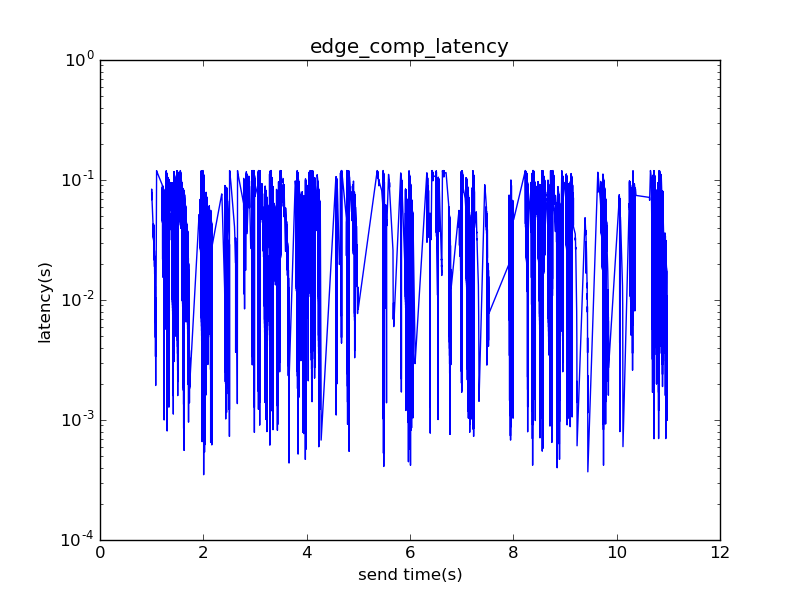
\includegraphics[width=8cm, height=6cm]{edgecomp_26}
\centering
\end{figure}
\begin{itemize}
	\item maximum latency experienced is \SI{.1182}{\second}
	\item minimum latency experienced is \SI{.00026}{\second} 
\end{itemize}

\end{frame}
\section{Experiment and Results}
\begin{frame}{Experiment and Results\big(Edge Computing\big)}
\begin{figure}
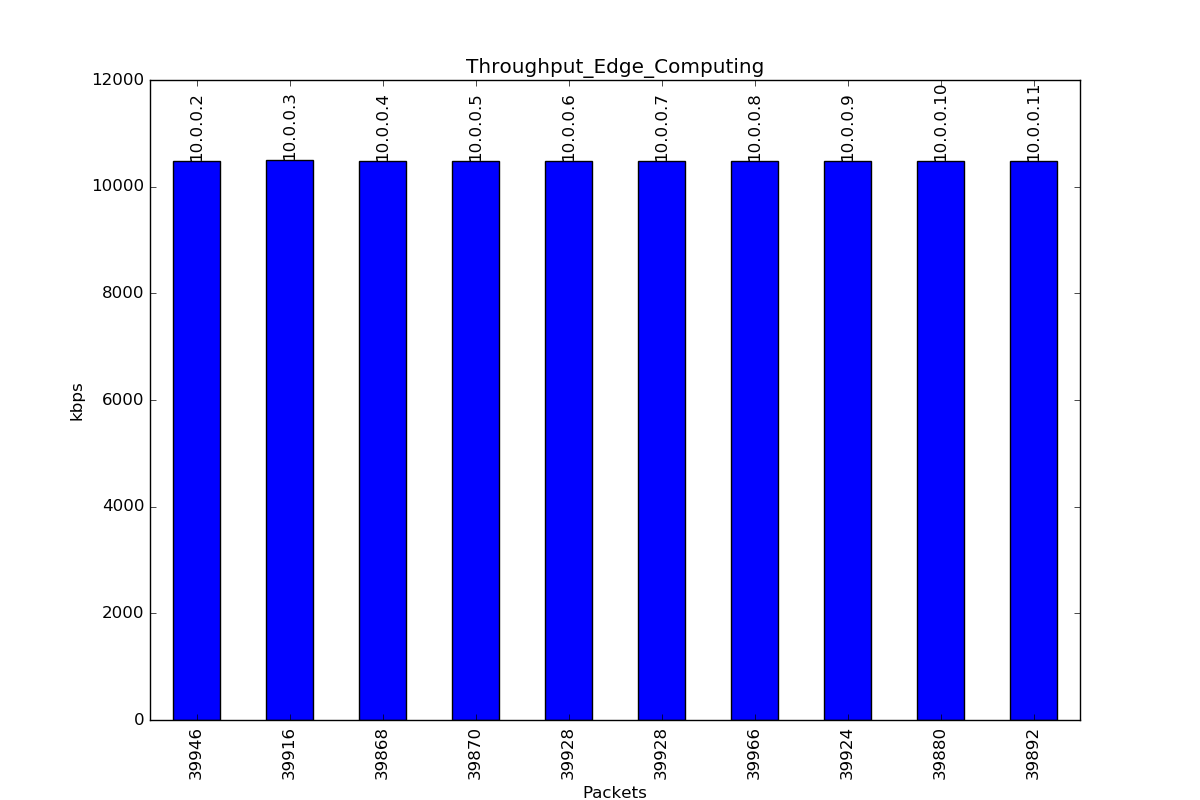
\includegraphics[width=8cm, height=6cm]{edgecompthrough}
\centering
\end{figure}
\begin{itemize}

	\item maximum throughput achieved is \SI{10.59}Mbps
	\item minimum throughput achieved is \SI{10.47}Mbps
	\item Average throughput achieved is \SI{10.48}Mbps
\end{itemize}

\end{frame}

\section{Experiment and Results}
\begin{frame}{Experiment and Results\big(Edge Cloud\big)}
\begin{figure}
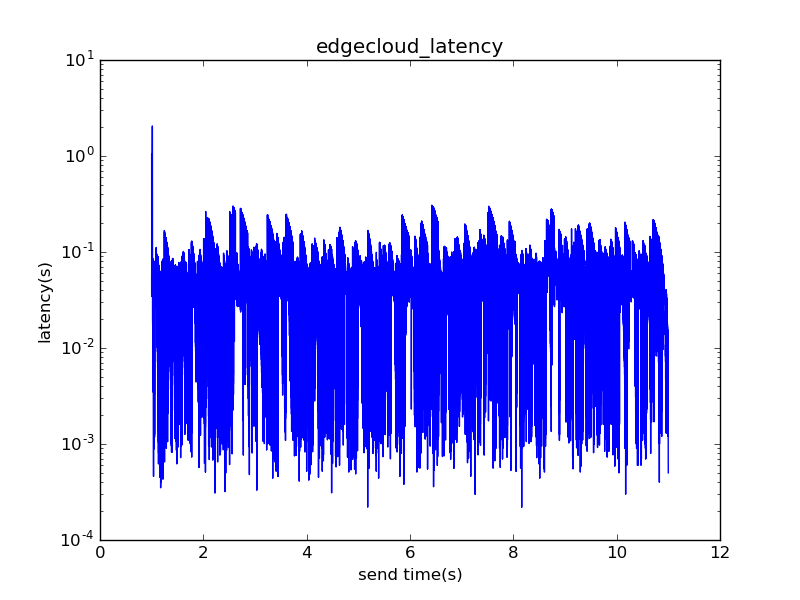
\includegraphics[width=8cm, height=6cm]{edgecloudlog26}
\centering
\end{figure}
\begin{itemize}
	\item maximum latency experienced is \SI{1.854}{\second}
	\item minimum latency experienced is \SI{.00043}{\second} 
\end{itemize}

\end{frame}
\section{Experiment and Results}
\begin{frame}{Experiment and Results\big(Edge Cloud\big)}
\begin{figure}
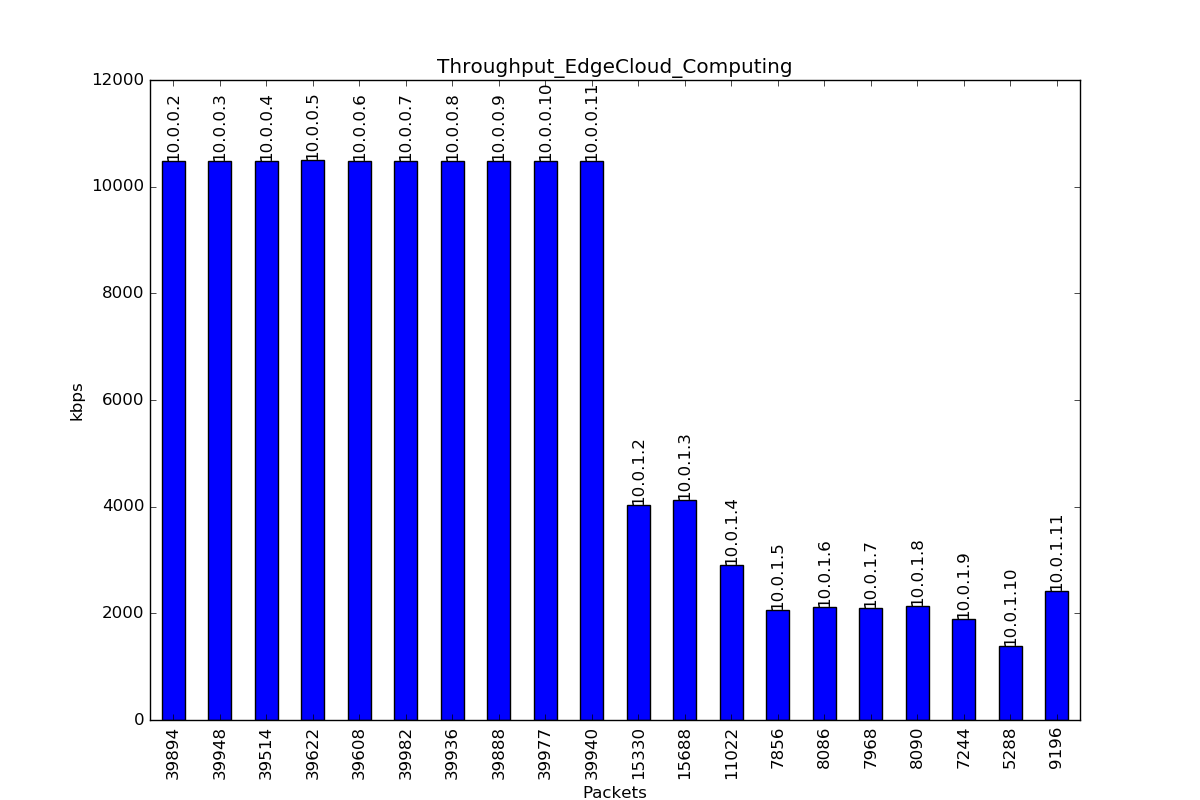
\includegraphics[width=8cm, height=6cm]{edgecloud}
\centering
\end{figure}
\begin{itemize}

	\item maximum throughput achieved is \SI{10.50}Mbps
	\item minimum throughput achieved is \SI{1.78}Mbps
	\item Average throughput achieved is \SI{6.51}Mbps
\end{itemize}

\end{frame}
\section{Experiment and Results}
\begin{frame}{Experiment and Results\big(Cloud Computing\big)}
\begin{figure}
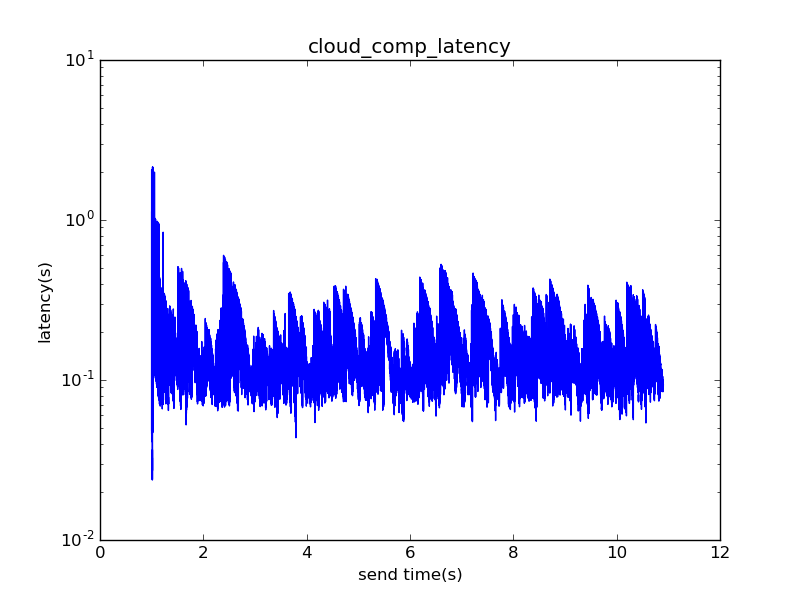
\includegraphics[width=8cm, height=6cm]{newcloudlatency}
\centering
\end{figure}
\begin{itemize}
	\item maximum latency experienced is \SI{2.145}{\second}
	\item minimum latency experienced is \SI{.0237}{\second} 
\end{itemize}

\end{frame}
\section{Experiment and Results}
\begin{frame}{Experiment and Results\big(Cloud Computing\big)}
\begin{figure}
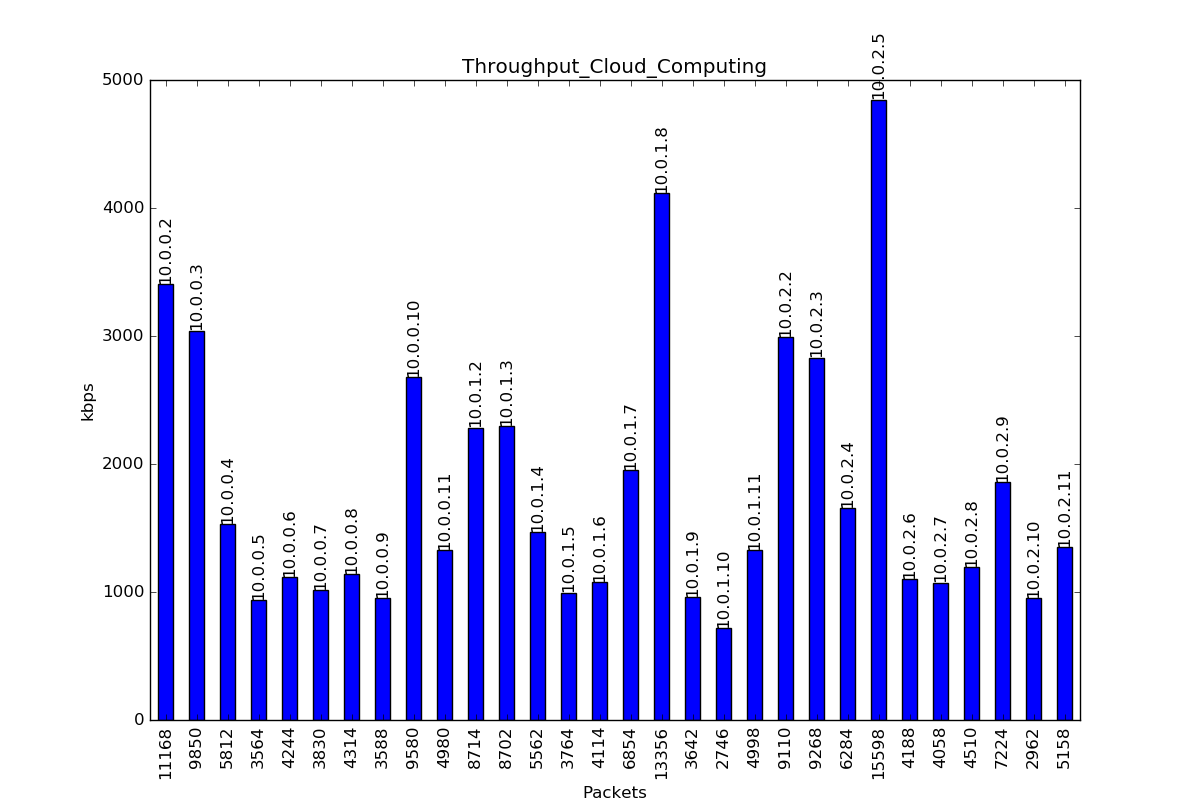
\includegraphics[width=8cm, height=6cm]{cloudth}
\centering
\end{figure}
\begin{itemize}

	\item maximum throughput achieved is \SI{4.87}Mbps
	\item minimum throughput achieved is \SI{0.721}Mbps
	\item Average throughput achieved is \SI{1.80}Mbps
\end{itemize}

\end{frame}
\section{Experiment and Results}
\begin{frame}{Experiment and Results}
\begin{table}
\centering
\caption{Comparison of different attributes}
\label{tab:table1}
\begin{tabular}{ |p{2.85cm}|p{2.5cm}|p{2cm}|p{2.5cm}|  }
 \hline
  Parameters & Edge \newline computing & Edge \newline Cloud & Cloud\newline Computing\\ 
 \hline
 Max Packets \newline sent \&\ received& 39966 & 39982 & 15598\\
 \hline
 Min Packets \newline sent \&\ received & 39868 & 9973 & 2746\\
 \hline
 Avg Packets \newline sent \&\ received & 39911 & 28703 & 6391 \\ 
 \hline
 Max \newline Throughput\big(Mbps\big) & 10.59 & 10.50 & 4.87\\
 \hline 
 Minimum \newline Throughput\big(Mbps\big) & 10.47 & 1.78 & 0.721 \\
 \hline
Average \newline Throughput\big(Mbps\big) & 10.48 & 6.51 & 1.80 \\
 \hline
\end{tabular}
\end{table}

\end{frame}
=======
	\item Here stations belong to two different wireless networks share a common cloud
	\item Implemented six wireless networks(each contains 4 stations) and 3 local servers.
	\item Maximum round trip time taken by node with ip address(10.0.0.7) is 38.137sec

\end{itemize}

\end{frame}
\section{Edge Cloud Topology}

\begin{frame}{Edge Cloud Topology}
\begin{itemize}
	\item Round trip time taken by nodes ranges from 34.99sec(ip address:10.0.0.1) to 38.137(ip address:10.0.3.5)
	\item Maximum delta time is .1032sec
	\item Total Packets(Packets A$\,\to\,$B and Packets B$\,\to\,$A) sent and received ranges from 632(316 in one direction) to 7000(3500 in one direction)
	\item Throughput ranges from 70k bps to 843k bps
	\item Average Throughput is 454k 
	

\end{itemize}
\end{frame}

\section{Cloud Computing Topology}

\begin{frame}{Cloud Computing Topology}
\begin{figure}
\includegraphics[width=7cm, height=4cm]{cloud_comp}
\centering
\end{figure}

\begin{itemize}
	\item Here all stations share a common cloud
	\item Implemented 3 wireless networks(each contains 6 stations) and a main server.
	\item Maximum round trip time taken by node with ip address(10.0.0.4) is 40.311sec

\end{itemize}

\end{frame}
\section{Cloud Computing Topology}

\begin{frame}{Cloud Computing Topology}
\begin{itemize}
	\item Round trip time taken by nodes ranges from 38.06sec(ip address:10.0.2.7) to 40.311(ip address:10.0.0.4)
	\item Maximum delta time is .832sec
	\item Total Packets(Packets A$\,\to\,$B and Packets B$\,\to\,$A) sent and received ranges from 698(349 in one direction) to 6276(3138 in one direction)
	\item Throughput ranges from 79k bps to 758k bps
	\item Average Throughput is 283k 
	

\end{itemize}
\end{frame}

\section{Results}
\begin{frame}{Results}
\begin{table}[h!]
\begin{center}
\caption{Comparison of different attributes}
\label{tab:table1}
\begin{tabular}{ |p{2.9cm}|p{2.5cm}|p{2cm}|p{2.5cm}|  }
 \hline
  & Edge \newline computing & Edge \newline Cloud & Cloud\newline Computing\\ 
 \hline
 Total Packets & 3293675 & 4200985 & 4294923\\
 \hline
 TCP \newline Retransmission \newline(packets)  & 294 & 5973 &8586\\
 \hline
 Lost Packets & 294 & 1794 & 2822 \\ 
 \hline
 Maximum \newline Throughput(Mbps) & 10.8 & 10.7 & 10.7\\
 \hline 
 Minimum \newline Throughput(Mbps) & 9.57 & 2.63 & 1.06 \\
 \hline
 Maximum \newline Latency & 1.03 & 3.0 &4.01 \\
 \hline
\end{tabular}
\end{center}
\end{table}

\end{frame}


>>>>>>> a768e6d35e5f5c2746483e50605e6bd25a5e7f09
\section{Conclusion}

\begin{frame}{Conclusion}
\begin{itemize}
<<<<<<< HEAD
	\item As expected,edge computing topology showed better results because of the dedicated servers for each wireless network
	\item Most of the stations in the cloud computing topology experienced high latency,less throughput 
=======
	\item As expected,edge computing topology showed better throughput,less round trip time and delta time
	\item Cloud computing could not perform well since the limitations of the channel bandwidth and high number of stations
>>>>>>> a768e6d35e5f5c2746483e50605e6bd25a5e7f09
\end{itemize}
\end{frame}
\end{document}


